\documentclass[a4paper]{article}

\usepackage[margin=0.5in]{geometry}
\usepackage{amsmath}
\usepackage{graphicx}
\usepackage{caption}
\usepackage{subcaption}
\usepackage[skip=2pt,labelfont=bf]{caption}

\newcommand{\scipnucaption}[1]{ Execution time for MKP having $#1$ constraint. }

\begin{document}

\centering{
  \large {\bf MKP Benchmark}: Branch-and-cut approach x Nemhauser-Ullman Algorithm \\
}

\begin{figure}[h]
  \centering
  \begin{subfigure}[t]{0.48\textwidth}
    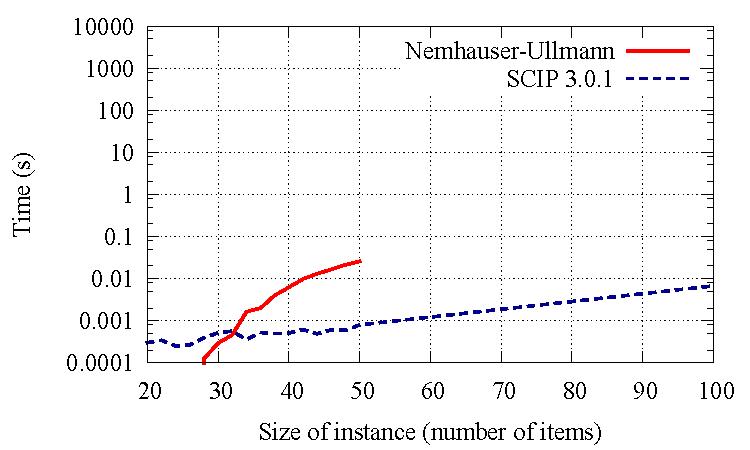
\includegraphics[width=\textwidth]{../../../experiments/mkp-scip-nu/plots/scip-nu-1}
    \caption{\scipnucaption{1}}
    \label{fig:gull}
  \end{subfigure}%
  \quad
  \begin{subfigure}[t]{0.48\textwidth}
    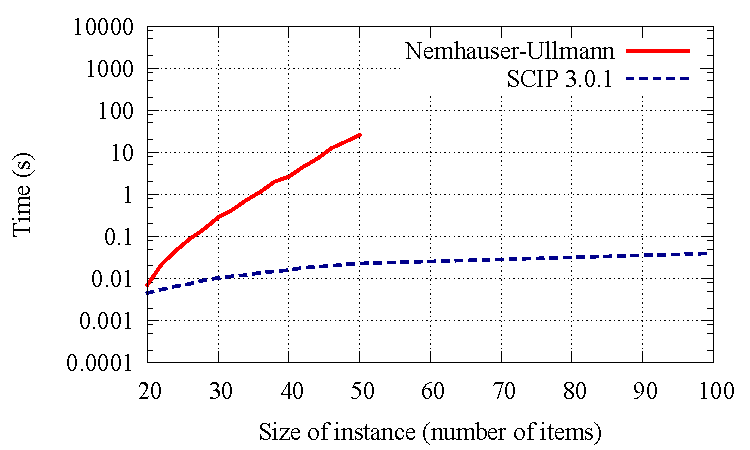
\includegraphics[width=\textwidth]{../../../experiments/mkp-scip-nu/plots/scip-nu-2}
    \caption{\scipnucaption{2}}
    \label{fig:tiger}
  \end{subfigure}
  \\ \vspace{12pt}
  \begin{subfigure}[t]{0.48\textwidth}
    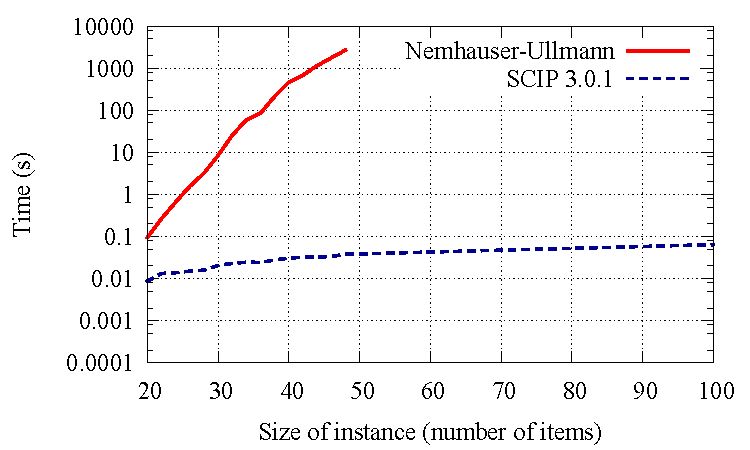
\includegraphics[width=\textwidth]{../../../experiments/mkp-scip-nu/plots/scip-nu-3}
    \caption{\scipnucaption{3}}
    \label{fig:mouse}
  \end{subfigure}
  \quad
  \begin{subfigure}[t]{0.48\textwidth}
    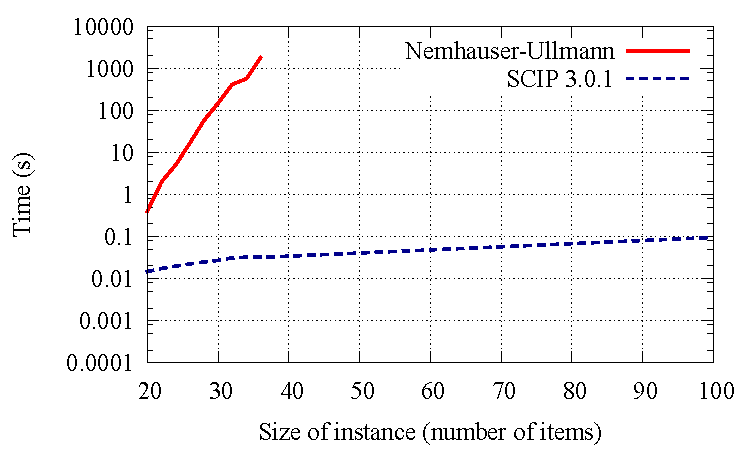
\includegraphics[width=\textwidth]{../../../experiments/mkp-scip-nu/plots/scip-nu-4}
    \caption{\scipnucaption{4}}
    \label{fig:mouse}
  \end{subfigure}
  \\ \vspace{8pt}
  \caption{Average running time for solving MKP instances
  using the Nemhause-Ullmann algorithm and SCIP solver.
  Each subfigure addresses a different number of constraint.
  The y-axis (time) is on logarithmic scale.
  }
  \label{fig:scip-nu}
\end{figure}

\end{document}


